\documentclass{scrartcl}
\usepackage[T1]{fontenc}
\usepackage[utf8]{inputenc}
\usepackage[ngerman]{babel}
\usepackage{amsmath,amssymb}
\usepackage{enumerate}
\usepackage{graphicx}
\usepackage{tabto}

\begin{document}
% Tab-Positionen
\TabPositions{0.8cm, 1.6cm, 2.4cm, 3.2cm}

\section*{Lösungen zum Thema Datenstrukturen}
\begin{enumerate}[(1)]

\item \begin{enumerate}[(a)]
\item
\begin{verbatim}
n=0:  /   n=1:  1    n=2:   1      n=3:      1           1
                            |               / \         / \
                            2              2   3       2   3
                            

n=4:     1          1         1         1         1
        / \        / \       / \       /         /  
       2   3      2   4     3   2     2         2
      /          /         /         / \       / \
     4          3         4         3   4     4   3
     
\end{verbatim}
\item Alle Heaps f\"ur $n\leq 3$, bei $n=4$ die ersten drei Heaps.
\item \begin{tabular}{|c|c|c|c|c|c|c|c|c|c|c|c|}
\hline
1 & 2 & 6 & 3 & $\bot$ & 8 & 7 & $\bot$ & $\bot$ & $\bot$ & $\bot$ & 9 \\ \hline
\end{tabular}
\end{enumerate}

\item 
Bemerkung: Die L\"osungen h\"angen nat\"urlich von der gew\"ahlten Datenstruktur ab. Dies ist nur eine m\"ogliche L\"osung.
\begin{enumerate}[(a)]
\item Doppelt verkettete Liste mit zus\"atzlichem Attribut $min$.
\item
\begin{verbatim}
add(L, x) //füge x in die Liste L ein
    // hier wäre der Code für das reine Einfügen in die Liste
    if x < L.min
    	L.min = x
    	
\end{verbatim}
\item
\begin{verbatim}
minimum(L) //gib Minimum aus L zurück
    return L.min
    	
\end{verbatim}
\item Falls das zu l\"oschende Element das minimale war, muss die komplette Liste nach dem neuen Minimum durchsucht werden. Die Laufzeit ist $\Theta(n)$. Bei einer normalen doppelt verketteten Liste w\"are das L\"oschen (bei Kenntnis des Pointers) aber in konstanter Zeit m\"oglich!
\end{enumerate}

\item
\begin{enumerate}[(a)]
\item Lösungsvorschlag: Hashtabelle mit Verkettung - Operationen laufen bei hinreichender Größe des Feldes in $O(1)$, Speicherplatz ist nicht beschränkt (außer durch Größe des Speichermediums).
\item Lösungsvorschlag: Warteschlange (Queue) - durch die FiFo-Strategie ändert sich die Reihenfolge der Anfragen beim Puffern nicht, außerdem werden ENQUEUE und DEQUEUE in jeweils konstantem Zeitaufwand ausgeführt.
\item Lösungsvorschlag: Max-Heap, da hier sowohl die Auswahl des Elements mit dem größten Schlüssel als auch das Einfügen neuer Prozesse hier besonders schnell ($O(log(n)$) erfolgen kann. 
\end{enumerate}

\item Skizze: \\
	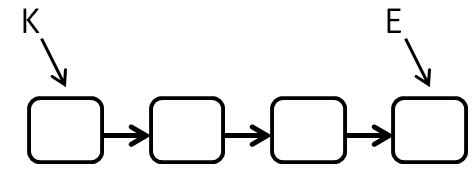
\includegraphics[width=6cm]{images/QueueListe}\\
	Anm: K muss auf den Listenanfang zeigen, da nur hier das Löschen in konstanter Zeit möglich ist.
\item \textit{ENQUEUE(x)}\\
	01 \tab \textbf{if} (E == \textit{NIL})\\
	02 \tab \tab E = x;\\
	03 \tab \textbf{else\\}
	04 \tab \tab  E.next = x;\\
	05 \tab \tab E = E.next;\\
	\ \\
	\textit{DEQUEUE()}\\
	01 \tab \textbf{if} (K == \textit{NIL})\\
	02 \tab \tab \textbf{error}(''Underflow!'');\\
	03 \tab \textbf{else}\\
	04 \tab \tab x = K;\\
	05 \tab \tab K = K.next;\\
	06 \tab \tab \textbf{return} x;

\end{enumerate}
\end{document}